% \bibliography{../src/bibliography}

This chapter introduces a neural Conditional Random Field (CRF) parser that can be used as an alternative proposal distribution for the approximate marginalization of the RNNG. This parser combines the efficient exact inference of chart-based parsing, the rich nonlinear features of neural networks, and the global training of a CRF. The chart-based approach allows efficient exact inference alowing for exact decoding and global sampling. The neural features can be complex and can condition on the entire sentence. And the CRF training objective [...something about receiving information about all substructures...]. The parser is an adaptation of the chart-based parser introduced in \citet{stern2017minimal} to global CRF training. The original is trained with a margin-based objective. Our interest in in this model is as a proposal distribution, which requires probabilistical training.

% \paragraph{Notation}
% Let a sentence be $x_1,\dots,x_n$, where each $x_i$
% is a word. We are given a CFG $(N, \Sigma, R, S)$ in Chomsky normal
% form. Let $\psi$ be a function that maps any rule production $r \in R$ of the form $\langle A \to B \;C, i, k, j \rangle$ or $\langle A, i, i+1 \rangle$ to a value $\psi(r) \geq 0$. Let a tree $T$ be a set of such rules $r$ with the only constraint that these rules make up a tree.

% I describe the probabilistic model of the parser.
% \begin{enumerate}
%   \item Introduce probabilistic model, reference the appendix on CRFs \ref{A3-crf}.
%   \item Desribe how this is an adaptation from \citet{stern2017minimal} to probabilistic training.
% \end{enumerate}

\section{Model}

The model is a CRF defined over labeled spans. We consider a tree as a collection of labeled spans $\y = \{ \y_a \}_{a=1}^A$ where $\y_a = \{ (i, j, \ell) }$, and define the score of a tree as the product of nonnegative local potentials $\Psi(\x, \y_a)$ that score these spans in conjunction with the sentence. The probability of a tree is the globally normalized score of the tree:
\begin{align}
  \label{eq:crf-model}
  p(\y \mid \x) &= \frac{1}{Z(\x)} \prod_{a=1}^A \Psi(\x, \y_a),
\end{align}
where
\begin{align*}
  Z(\x) = \sum_{ \y \in \yieldx } \prod_{a=1}^A \Psi(\x, \y_a)
\end{align*}
is the normalizing constant that sums over all the possible parse trees and makes sures that the probability distribution sums to 1. This normalizing constant can be computed efficiently with the inside algorithm.

The factorization over labeled spans is an even stronger assumption than that typically made of factorization over anchored context-free rules. By scoring just labeled spans, the scoring function has no access to information about child nodes. This puts a greater burden on the scoring function, which is made up for by a very rich neural network parametrization, but will also greatly reduce the size of the state-space of the dynamic programs, greatly speeding up training and inference.

\subsection{Features}
The scoring function $\Psi$ is implemented using neural networks following \citet{stern2017minimal}. Although the local potentials can only make minimal use of structural information, as we argued above, they can depend on the entire sentence. This suggest the use of $\rnn$ encodings.

The representation of a span $(i, j)$ is the concatenation of the difference between forward and backward vectors computed by a bidirectional $\rnn$
\begin{align}
  \label{eq:potential-function}
  \vecs_{ij} = [\fw_j - \fw_i; \bw_i - \bw_j],
\end{align}
illustrated in figure \ref{fig:span-feature}. The score for a label is computed from this vector using a feedforward network:
\begin{align}
   % s(i, j, \ell) = s(i, j) = \Big[ \ff( \vecs_{ij} ) \Big]_{\ell}.
  \log \Psi(\x, \y_a) = \Big[ \ff( \vecs_{ij} ) \Big]_{\ell}.
\end{align}

\begin{figure}
  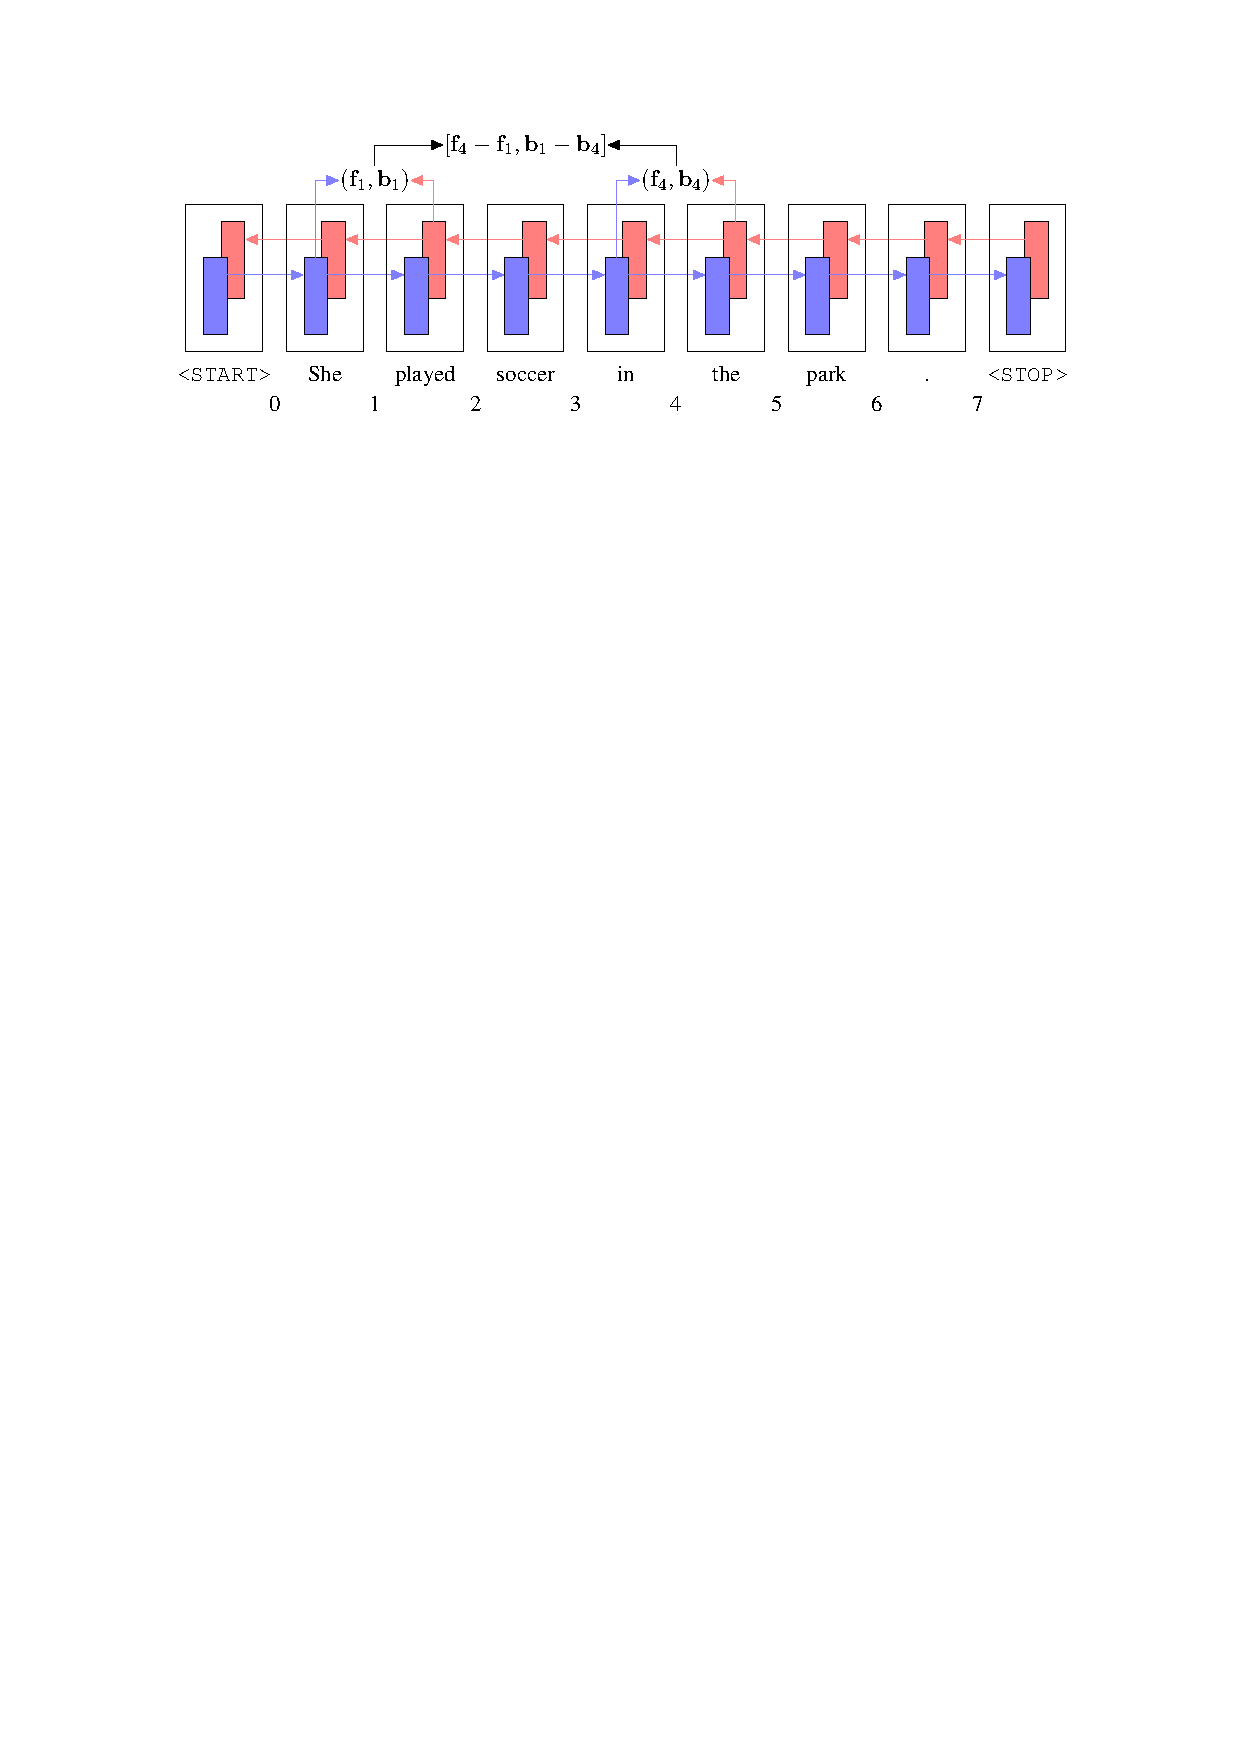
\includegraphics{span-encoding.pdf}[width=\textwidth]
  \caption{Representation for the span $(1, 4)$ computed from $\rnn$ encodings. Taken from \citet{stern2018analyis}.}
  \label{fig:span-feature}
\end{figure}

\subsection{Motivation}
\begin{itemize}
  \item Key point to make: this model regards a constituency tree as a collection of \textit{labeled spans} over a sentence. Earlier models, both log-linear and neural, regard a constituency tree as a collection of \textit{anchored rules} over a sentence \citep{finkel2008crf,klein2015crf}.
  \item A model over spanned rules puts more expressiveness in the state space of the dynamic program, because the correlations between subparts of the trees are modeled through the rich rules. The model in \citet{stern2017minimal} instead puts the expressiveness in the input space by using rich neural feature representations. The state space in contrast is less structured, because the score-function is agnostic to the composition of it's children.
  \item Earlier approaches went even farther. These approaches enriched the grammar by lexicalizing the rules \citep{collins2003head} or by breaking the grammar's independence assumptions by annotating the rule with parent and sibling labels \citep{klein2003accurate}.
  \item The choice to model labeled spans makes dramatically improves the speed of this model. In the section on inference we will show precisely how.
\end{itemize}

\section{Inference}
Due to the parametrization, the model allows efficient inference. In this section we describe efficient solutions to three related problems:
\begin{itemize}
  \item Find the best parse $\mathbf{y}^{*} = \arg \max_{\mathbf{y}} p(\mathbf{y} | \mathbf{x})$
  \item Compute the normalizer $Z(\mathbf{x}) = \sum_{ \mathbf{y} } \prod_{ a=1 }^{ A } \Psi( \mathbf{x}, \mathbf{y}_a )$, where $F = \{ \Psi_a \}_{a=1}^{A}$ is the set of factors in the graph.
  \item Compute the entropy conditioned on $\mathbf{x}$, $H(\mathbf{y} | \mathbf{x})$.
\end{itemize}
All three problems can be solved with a different instance of the same two algorithm: the inside algorithm and the outside algorithm.

\subsection{Inside recursion}
% NOTE: This is a complete draft section, just for me to get the correct derivation for the implementation. In the actual section I will follow the semiring formulation, and connect it with the belief-propagation/message-passing/sum-product algorithm.
%
In this derivation we follow Michael Collins notes on the Inside-Outside Algorithm.\footnote{\url{http://www.cs.columbia.edu/~mcollins/io.pdf}} We have the following general result for the inside value $\alpha$. For all $A \in N$, for all $0 \leq i < n$
\begin{align}
    \label{eq:collins-inside-base}
    \alpha(A,i,i+1) = \psi(A, i, i+1)
\end{align}
and for all $(i, j)$ such that $1 \leq i < j \leq n$:
\begin{align}
    \label{eq:collins-inside-general}
    \alpha(A,i,j) = \sum_{A \to B C} \sum_{k=i+1}^{j-1} \psi(A \to B \;C, i, k, j) \cdot \alpha(B,i,k) \cdot \alpha(C,k,j)
\end{align}
% \begin{align}
% \label{eq:rule-score}
%     \log\psi(A \to B \;C, i, k, j) \defeq s(i, j, A) + s_{span}(i, k) + s_{span}(k, j),
% \end{align}
Note that we are considering a CFG in which the rule set is complete, i.e.
\begin{align}
  \langle A \to B \;C \rangle \in R \text{ for each } (A, B, C) \in N^3,
\end{align}
and recall that the labels $B$ and $C$ do not appear in the scoring functions in \ref{eq:rule-score}. These facts will allow us to simplify the expression in formula \ref{eq:collins-inside-general} as
\begin{subequations}
\begin{align*}
    \alpha(A,i,j) &= \sum_{B \in N} \sum_{C \in N} \sum_{k=i+1}^{j-1} \tilde{s}(i, j, A) \cdot \alpha(B,i,k) \cdot \alpha(C,k,j) \\
        &= \tilde{s}(i, j, A) \cdot \sum_{k=i+1}^{j-1} \sum_{B \in N} \alpha(B,i,k) \cdot \sum_{C \in N} \alpha(C,k,j) \\
        &= \tilde{s}(i, j, A) \cdot \sum_{k=i+1}^{j-1} S(i,k) \cdot S(k,j) \label{eq:final-inside}
\end{align*}
\end{subequations}
where we've introduced a number of notational abbreviations
\begin{align*}
  \tilde{s}(i, j, A)
    &= \exp( s(i, j, A) ) \\
    S(i,j) &= \sum_{A \in N} \alpha(A,i,j)
\end{align*}
Note that this is the exact same formula as \ref{eq:inside-semiring}.

From equation \ref{eq:final-inside} we can deduce that we in fact do even need to store the values $\alpha(i, j, A)$ but that it suffices to only store the marginalized values $S(i, j)$. In this case, the recursion simplifies even further:
\begin{subequations}
\begin{align*}
    S(i, j) &= \sum_{A \in N} \alpha(A,i,j) \\
        &=  \sum_{A \in N} \tilde{s}(i, j, A) \cdot \sum_{k=i+1}^{j-1} S(i,k) \cdot S(k,j) \\
        &= \Bigg[ \sum_{A \in N} \tilde{s}(i, j, A) \cdot \Bigg] \Bigg[\sum_{k=i+1}^{j-1} S(i,k) \cdot  S(k,j) \Bigg]
\end{align*}
\end{subequations}
where we put explicit brackets to emphasize that independence of the subproblems of labeling and splitting. We can now recognize this as the `inside' equivalent of the expression from the paper\footnote{I believe there is actually an error in this equation: it should read  $s(i, j, \ell) + s_{span}(i, j)$ instead of just $s(i, j, \ell)$. This is implied by the score for a single node, which is given by equation \ref{eq:rule-score}, taken directly from the paper.}
\begin{align}
    s_{best}(i, j) = \max_{\ell} [s(i, j, \ell)] + \max_{k}[ s_{split}(i, k, j)].
\end{align}
The recursions are the same; the semirings are different. The viterbi recursion given above is in the \textsc{ViterbiSemiring}, which uses the $\max$ operator as $\oplus$; the inside recursion given in \ref{eq:final-inside} has standard addition (+) instead.


\subsection{Outside recursion}
\begin{align*}
    \beta(A, i, j) &= \sum_{B \to C A \in R} \sum_{k=1}^{i-1} \psi(B \to C A, k, i-1, j) \cdot \alpha(C, k, i-1) \cdot \beta(B, k, j) \\
            &\qquad + \sum_{B \to A C \in R} \sum_{k=j+1}^{n} \psi(B \to A, C, i, j, k) \cdot \alpha(C, j+1, k) \cdot \beta(B, i, k) \\
        &= \sum_{B \in N} \sum_{C \in N} \sum_{k=1}^{i-1} \psi(B, k, j) \cdot \alpha(C, k, i-1) \cdot \beta(B, k, j) \\
            &\qquad + \sum_{B \in N} \sum_{C \in N} \sum_{k=j+1}^{n} \psi(B, i, k) \cdot \alpha(C, j+1, k) \cdot \beta(B, i, k) \\
        &=  \sum_{k=1}^{i-1}  \Bigg[ \sum_{B \in N} \psi(B, k, j)  \cdot \beta(B, k, j) \Bigg] \cdot \Bigg[ \sum_{C \in N} \alpha(C, k, i-1) \Bigg] \\
            &\qquad + \sum_{k=j+1}^{n}  \Bigg[ \sum_{B \in N}  \psi(B, i, k) \cdot \beta(B, i, k) \Bigg] \cdot  \Bigg[ \sum_{C \in N} \alpha(C, j+1, k) \Bigg] \\
        &=  \sum_{k=1}^{i-1}  S'(k, j) \cdot S(k, i-1) + \sum_{k=j+1}^{n} S'(i, k) \cdot  S(j+1, k) \\
\end{align*}
where
\begin{align*}
    S(i, j) &= \sum_{A \in N} \alpha(A, i, j) \\
    S'(i, j) &= \sum_{A \in N} \psi(A, i, j) \beta(A, i, j)
\end{align*}

\section{Experiments}
We perform three types of experiments with the CRF parser:
\begin{itemize}
  \item We show that the model is a good supervised parser. We train the model supervised on the PTB and show the f-score on the PTB test set.
  \item We evaluate the joint RNNG with samples from the CRF parser. We compare the perplexity and fscore with RNNG case.
  \item We evauluate `how good the model is' as a sampler.
\end{itemize}

\paragraph{Supervised model} We investigate the following.
\begin{itemize}
  \item We have some optimization and hyperparameter choices here. The original paper uses Adam with 0.001 and a LSTM of dimension 250, which gives the model around 2.5 million parameters. For the discriminative RRNG we use SGD with 0.1, and hidden sizes of 128 gives the model around 800,000 parameters.
  \item I suggest two experiments: (1) use the default setting from \citep{stern2017minimal} and (2) use the settings for the RNNG with a hidden size to match the 800,000 parameters.
\end{itemize}

\paragraph{Proposal model} We investigate the following:
\begin{itemize}
  \item We evaluate validation F-score and perplexity.
  \item We evaluate F-score with 100 samples (as many proposal trees as possible).
  \item We evaluate perplexity with varying number of samples: 1 (argmax), 10, 20, 50, 100 (default). The peplexity evaluation with the argmax prediction gives an impression of the uncertaty in the model \citep{buys2018exact}.
  \item  We perform learning rate decay and model selection based on a development score computed with the samples from the discriminative RNNG. Undecided: should we train a separate joint RNNG with CRF samples?
\end{itemize}

\paragraph{Sampler} We investigate the following:
\begin{itemize}
  \item We asses the conditional entropy of the model. This is most quantitative. Recall that conditional entropy is defined as
  \begin{equation}
    \text{H}(Y|X) = \sum_{x \in \mathcal{X}} p_X(x)\text{H}(Y|X = x),
  \end{equation}
  where
  \begin{equation}
    \text{H}(Y|X = x) = - \sum_{y \in \mathcal{Y}} p_{Y|X}(y|x) \log p_{Y|X}(y|x).
  \end{equation}
  The quantity $\text{H}(Y|X = x)$ can computed exactly with the CRF parser. We estimate the quantity $\text{H}(Y|X)$ by a sum over the development dataset. For the probabilities $p_X(x)$ we use the marginalized probabilities of the joint RNNG (with samples from the CRF parser $p_{Y|X}$).
  \item We asses for some cherry picked sentences. This is more qualitative. These sentences should be difficult or ambiguous. Or they can be ungramatical when taken from the syneval dataset. We can evaluate their entropy, and the diversity of samples, for example to see if there are clear modes. We can make violinplots of the probabilities of the samples. We can compute the f-scores of the samples compared with the argmax tree.
\end{itemize}

\section{Related work}
Here I describe related work, and in particular earlier approaches to (neural) CRF-parsing.
\begin{enumerate}
  \item Of course \citep{stern2017minimal}
  \item CRFs \citep{sutton2012crf}
  \item CRF parsing with linear and nonlinear features \citep{finkel2008crf,klein2015crf}
  \item Attempts to simplify the grammar and thus the state-space of the dynamic program \citep{hall2014less}.
  \item Recent extension of \citet{stern2017minimal}, with same model but different features \citep{kitaev2018attentive}.
\end{enumerate}

Earlier work on CRF parsing consider a tree as a collection of anchored rule productions productions \cite{finkel2008crf,klein2015crf}, and hence define the score of a tree as the product over clique potentials on anchored rules:
\begin{align}
  \log\psi(A \to B \;C, i, k, j) = \log\psi(A, i, j)\\
\end{align}
discarding the rest of the span information. The function is then defined as
\begin{align}
  \label{eq:span-score}
  \log\psi(A, i, j) &\defeq s(i, j, A),
\end{align}
and thus the potential of a tree as
\begin{align}
\label{eq:tree-score}
    \log\Psi(T) &= \sum_{r \in T} \log\psi(r) \\
      &= \sum_{\langle A, i, j \rangle \in T} s(i, j, A), \\
\end{align}
Note that the potential function as defined in \ref{eq:rule-score} disregards most of the information in a binary rule. In particular we see that $B$, $C$ and $k$, the labels and split-point of the children, are discarded.

Now note that equation \ref{eq:tree-score} corresponds exactly to the second formula in section 3 of the minimal span-based parser paper
\begin{align}
s_{tree}(T) = \sum_{(\ell(i,j))\in T}[s(i, j, \ell)] .
\end{align}
which is how I derived that \ref{eq:rule-score} is the correct formula for the rule score.


% \section{Semiring formulation}
% So yeah, the highlights are: an edge connects three nodes, a parent and two \textsc{children}, each node is a labelled \textsc{span}; you need to identify the scoring function for an edge, let’s call it $w(e)$,  in this case we have
% \begin{align}
%     w(e) = f(\textsc{head}(e)) \bigotimes_{c \in \textsc{children}(e)} g(\textsc{span}(c))
% \end{align}
% where $f$ and $g$ are parametric functions; then you can compute the Inside recursion for a node v
% \begin{align}
%     I(v) = \bigoplus_{e \in BS(v)} w(e) \otimes \bigotimes_{c \in \textsc{children}(e)} I(c)
% \end{align}
% where I’m using $BS(v)$ to denote the set of edges incoming to $v$; note that BS here basically enumerates the different ways to segment the string under $(i,j)$ into two adjacent parts and the different labels of each child \textsc{span} (let’s call these $a$ and $b$, each an element in the labelset $L$), thus we can write
% \begin{align}
% I(v=[i,j,l]) = \bigoplus_{ \substack{ e=[i,j,l,k,a,b]: \\ a \in L, \\ b \in L, \\ k \in \{i+1,...,j-1\} } } w(e) \otimes I([i,k,a]) \otimes I([k+1,j,b])
% \end{align}
% Now the key is to realise that $w(e)$ factorises and therefore we can rewrite this as
% \begin{align}
%     I(v=[i,j,l]) = f(i,j,l) &\otimes \bigoplus_{k=i+1}^{j-1} g(i,k) \otimes g(k+1,j) \\
%         &\otimes \bigoplus_{a \in L}  I([i,k,a]) \\
%         &\otimes \bigoplus_{b\in L} I([k+1,j,b])
% \end{align}
% and this finally motivates having an inside table for the \textsc{span}s (with labels summed out), let’s call that
% \begin{align}
%     S(i,j) = \bigoplus_{l \in L} I(i,j,l)
% \end{align}
% and then we have the result
% \begin{align}
% \label{eq:inside-semiring}
%     I(i,j,l) = f(i,j,l)\otimes \bigoplus_{k=i+1}^{j-1} g(i,k)\otimes g(k+1,j) \otimes S(i,k) \otimes S(k+1,j).
% \end{align}
